% 7.3：依据表5及同源的60 s采样场分析长期干燥特征；图7使用用户提供的两张PNG。
\subsection{结果分析}
\label{sec:p3-analysis}

\subsubsection{末期减速及扩散能力衰减}

由表\ref{tab:p3C}估算，中心含水率在$6$--$12\ \mathrm{h}$内下降$0.5609\cunit$，
而在$48$--$54\ \mathrm{h}$内仅下降$0.0079\cunit$。
\textbf{两个时间窗等长，前者的平均下降速率约为后者的70倍} ，
与图\ref{fig:p3-drying}(a)后期曲线趋平的现象一致。

$6\ \mathrm{h}$后温度已基本稳定在$50\tempunit$附近。
将未舍入状态代入式\eqref{eq:p2-properties}，表面扩散系数由$6\ \mathrm{h}$时约
$6.91\times10^{-9}\ \mathrm{m^2/s}$降至$54\ \mathrm{h}$时约
$3.29\times10^{-12}\ \mathrm{m^2/s}$。
低含水率外层的扩散能力减弱，连同表面交换驱动力的下降，使持续脱水受限，
因而\textbf{不能按前期速率线性外推终点}。

\begin{figure}[!htbp]
\centering
% 保持原图7的0.98\textwidth宽度及264.5905/633.317547高宽比。
% 统一裁去两张PNG的白边，完整保留上方结束时间与右侧烘干判据。
% trim按源PNG的300 dpi换算；仅指定宽度以保持原比例，两图的轴框上下对齐。
\setlength{\unitlength}{0.98\textwidth}
\begin{picture}(1,0.417784887)
  \put(0,0.031758297){\makebox(0,0)[lb]{%
    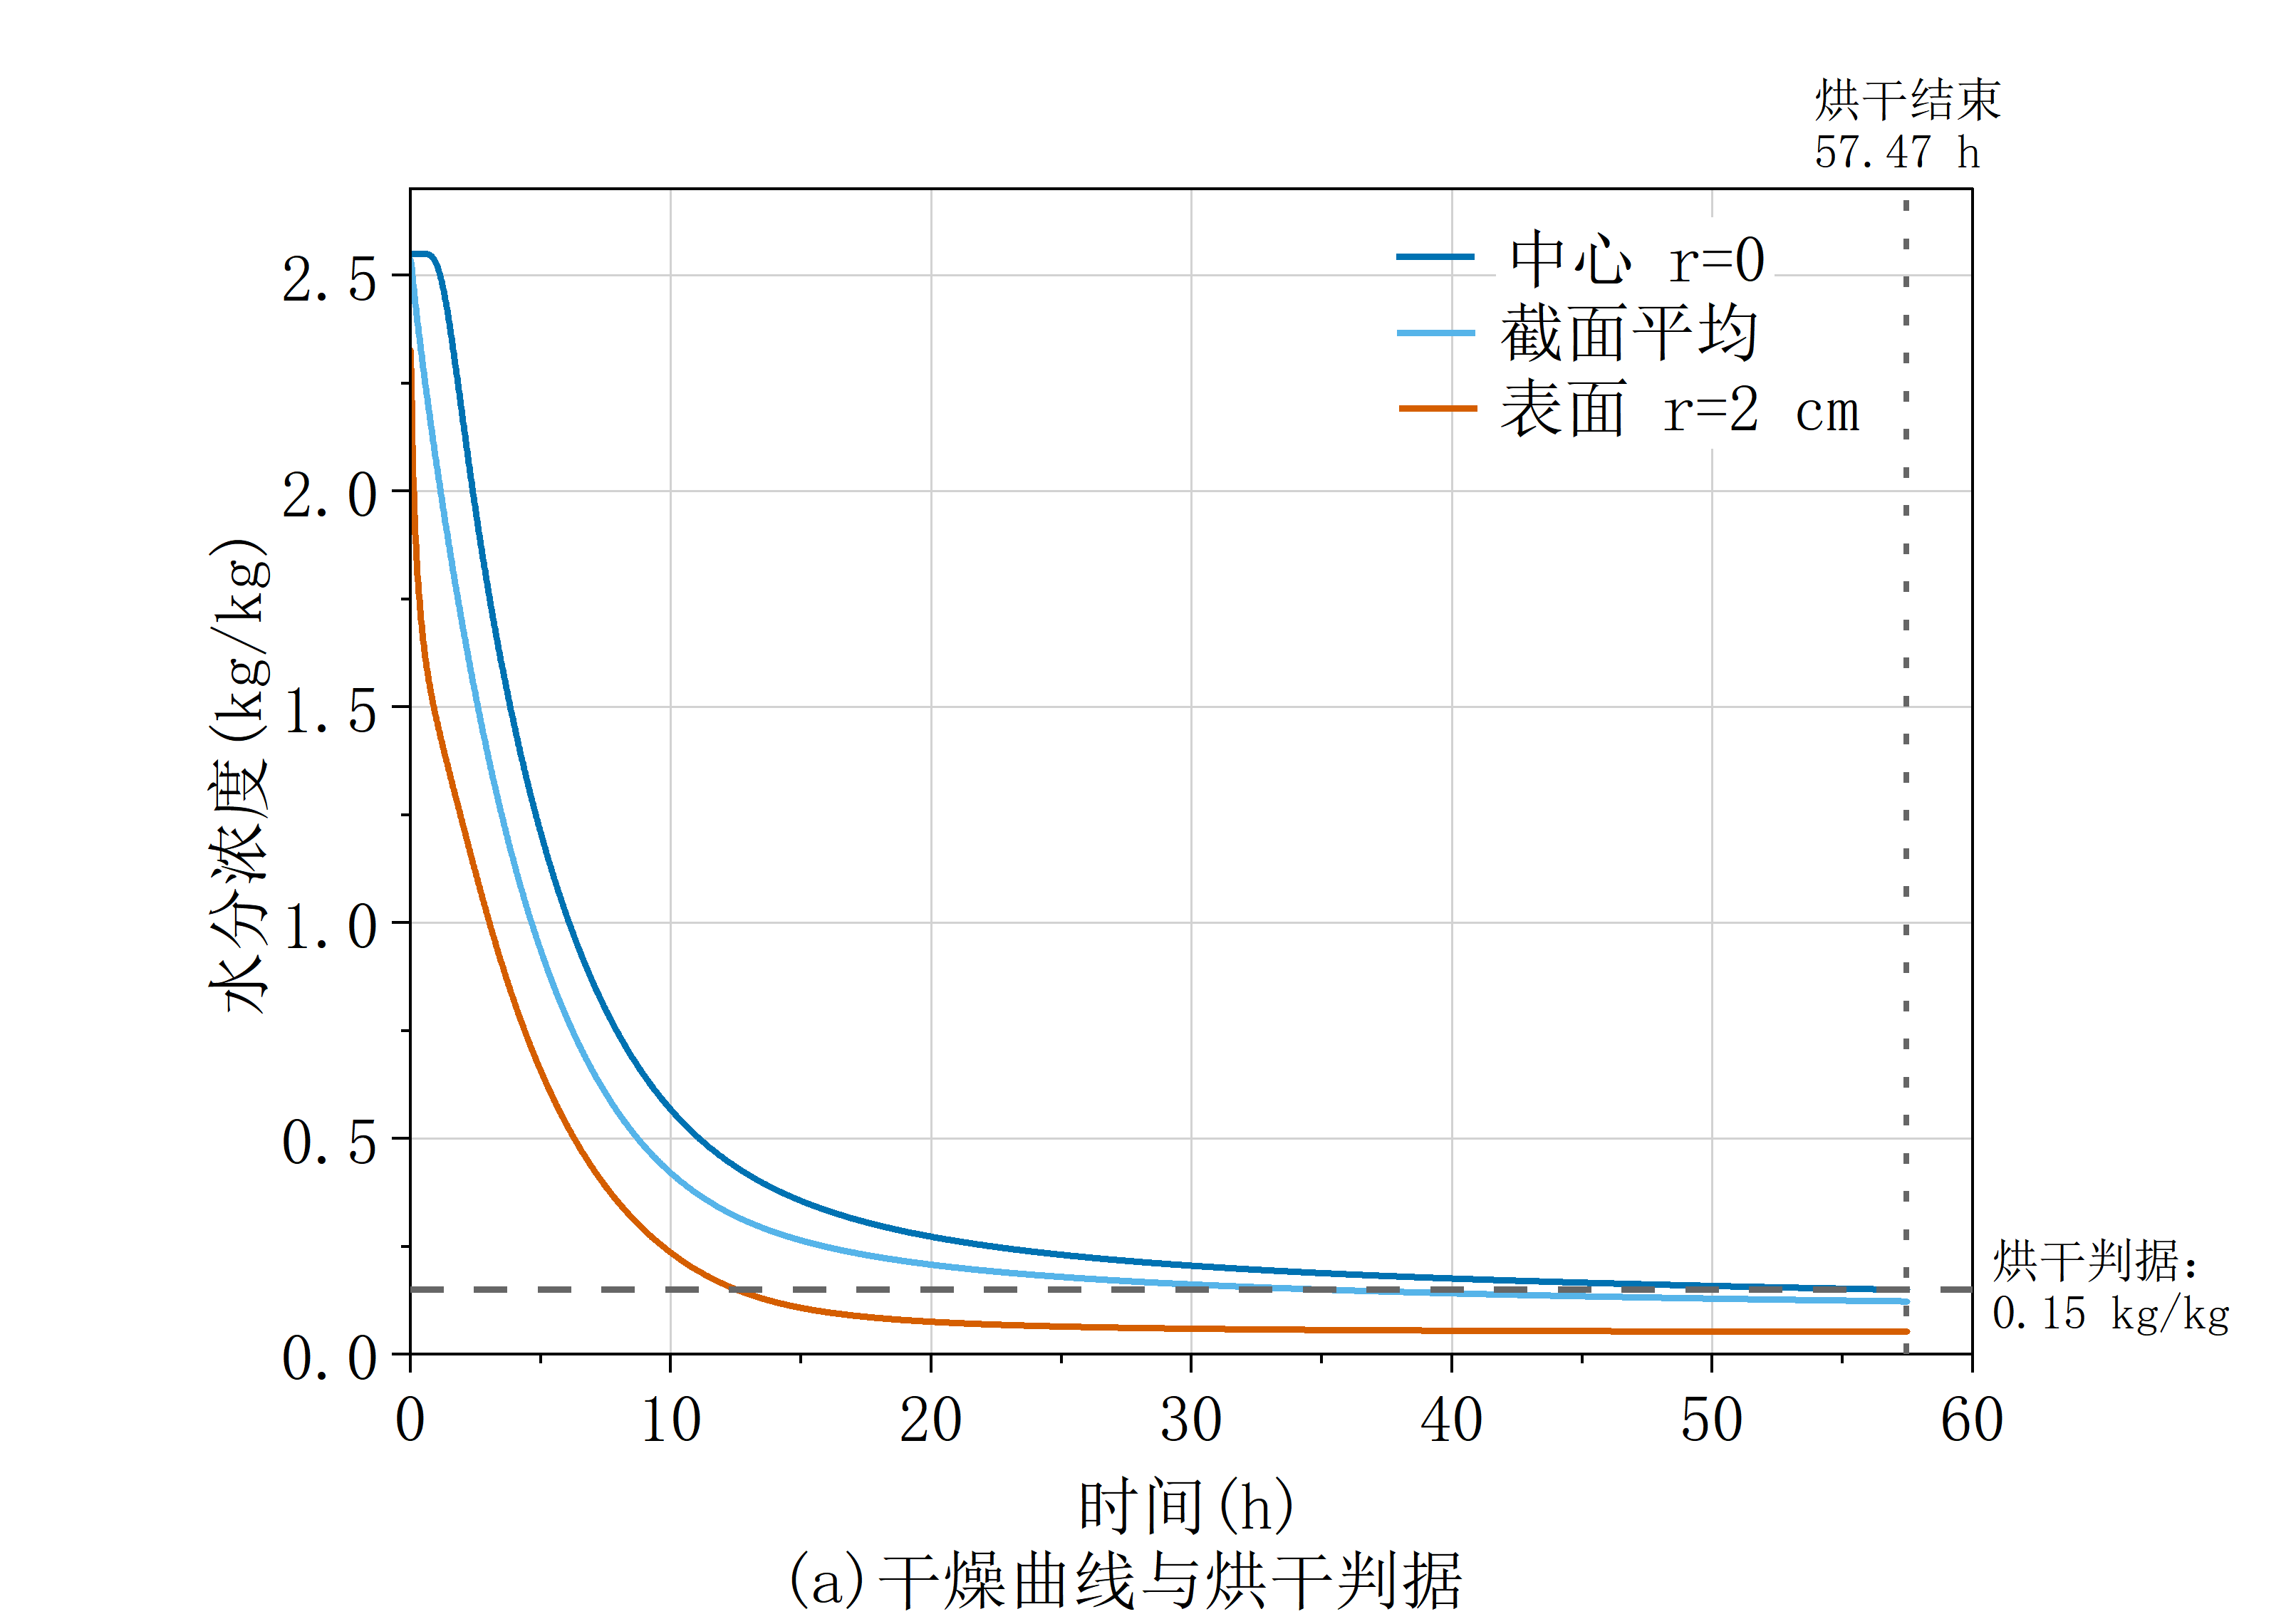
\includegraphics[trim={66.000bp 26.400bp 17.040bp 22.800bp},clip,
      width=0.49\unitlength]{图8(a).png}}}
  \put(0.51,0.031758297){\makebox(0,0)[lb]{%
    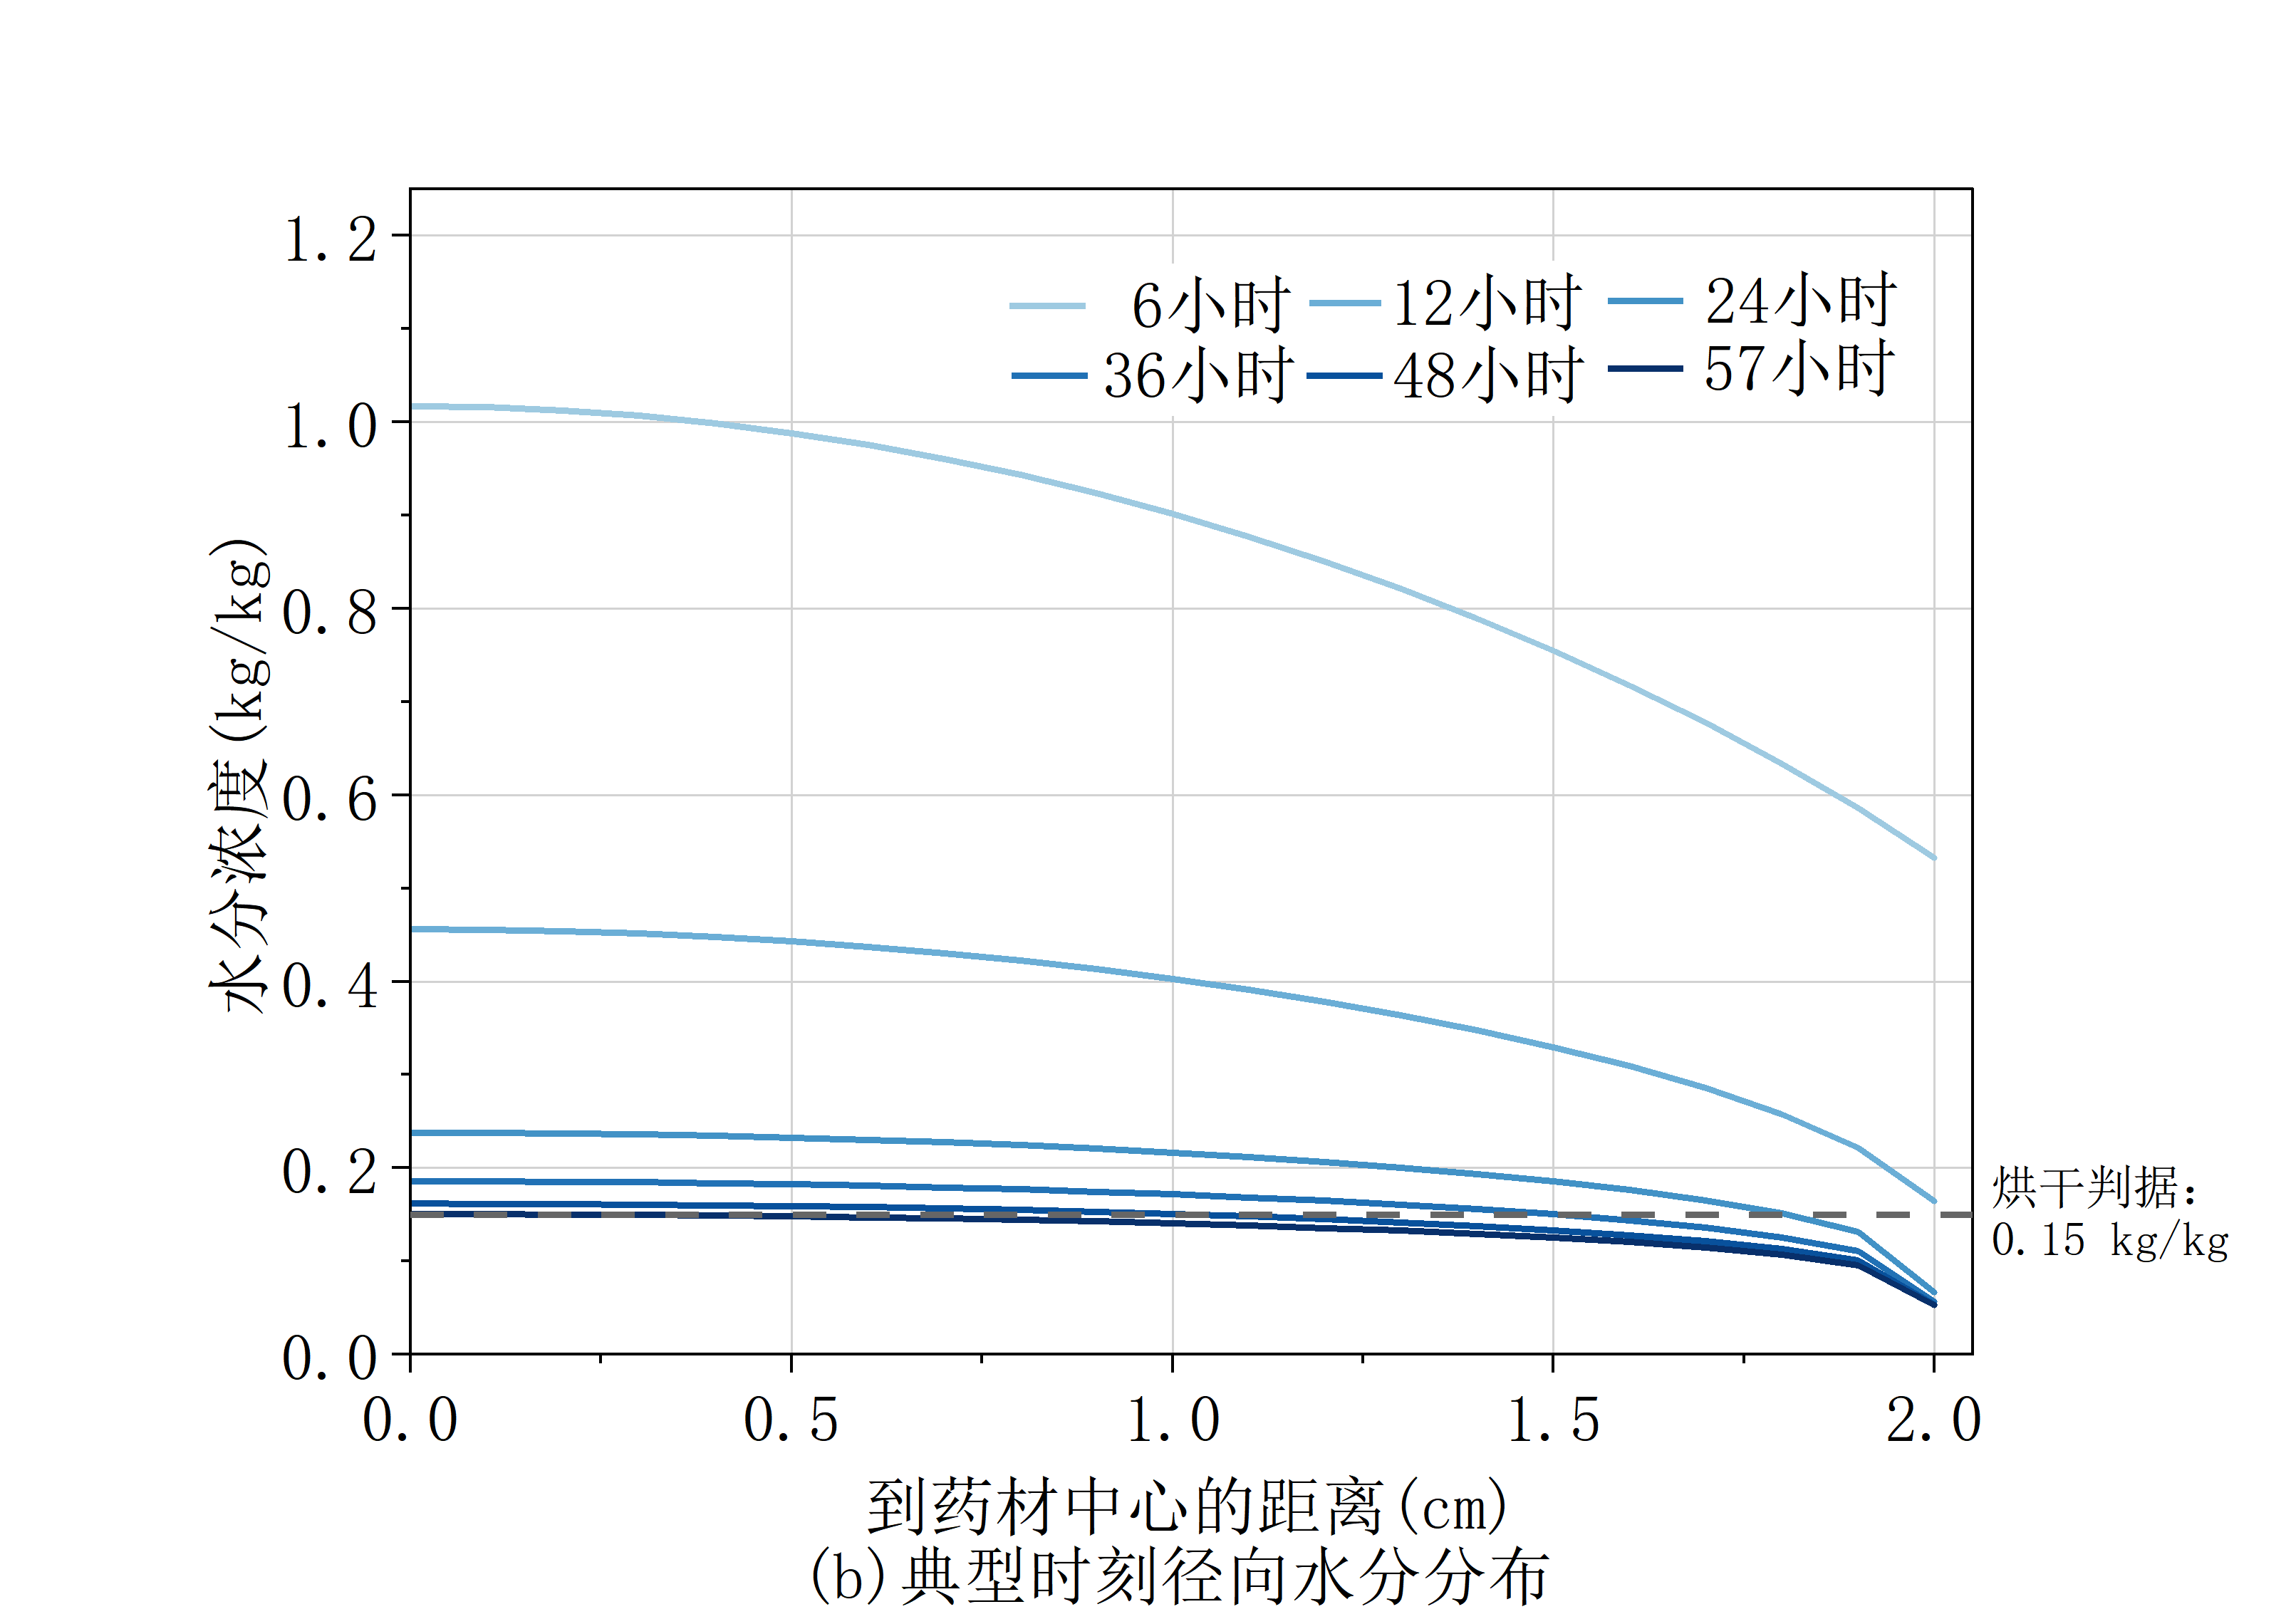
\includegraphics[trim={66.000bp 26.400bp 17.040bp 22.800bp},clip,
      width=0.49\unitlength]{图8(b).png}}}
\end{picture}
\caption{问题三全程干燥曲线与代表时刻的径向含水率分布}
\label{fig:p3-drying}
\end{figure}

\subsubsection{中心控制终点与径向差异}

在约$12.57\ \mathrm{h}$的保存结果中，表面含水率已低于$0.15\cunit$，
中心仍约为$0.4323\cunit$；图\ref{fig:p3-drying}(a)中的截面平均曲线也先于中心越过限值。
全域达标的临界时长则为$57.4721\ \mathrm{h}$，较表面达标滞后约$45 \mathrm{h}$。因此，\textbf{表面干燥不能代表整体达标，内部残余水分的缓慢迁出决定了烘干过程的长尾。}
结合第\ref{sec:p3-solution}节的逐节点核验，\textbf{中心是本算例的终点控制位置}。
$57.4721\ \mathrm{h}$的临界状态下，中心和表面含水率分别为
$0.1500\cunit$、$0.0527\cunit$，仍存在径向差异，
表明到达临界时刻并不意味着内部含水率已经均匀。
